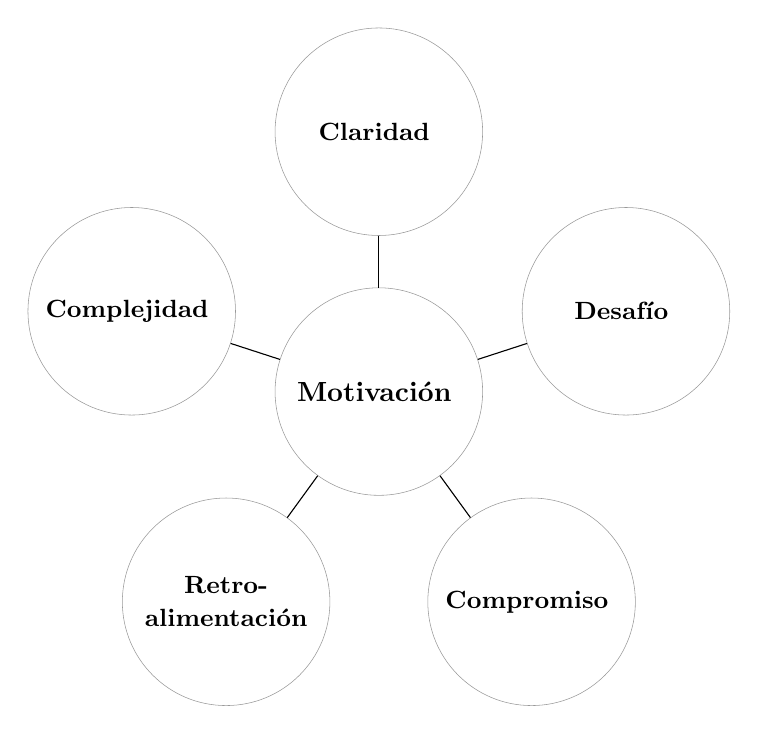
\begin{tikzpicture}[
		every node/.append style={circle,draw=gray!80,align=center,minimum width=75pt,very thin}
  	]
	\node[] (L) at (90:3.3) {
		\textbf{\small Claridad}
	};
	\node[] (D) at (18:3.3) {
		\textbf{\small Desafío}
	};
	\node[] (J) at (162:3.3){
		\textbf{\small Complejidad}
	};
	\node[] (R) at (234:3.3){
		\textbf{\small Retro-}\\\textbf{\small alimentación}
	};
	\node[] (C) at (306:3.3){
		\textbf{\small Compromiso}
	};
	\node[] (M) at (0,0){
		\textbf{Motivación}
	};
	\draw[-] (L) edge (M);
	\draw[-] (D) edge (M);
	\draw[-] (J) edge (M);
	\draw[-] (R) edge (M);
	\draw[-] (C) edge (M);
\end{tikzpicture}
